\newprob{1718634067}
{
    % Active Physics p79 q1
    以下哪些是放射性示蹤物的用途?
    \begin{tasks}
        \task 檢查地下喉管出現滲漏的位置
        \task 探究植物攝取養分的過程
        \task 研究消化食物的過程
        \task 以上皆可
    \end{tasks}
}{D}

\newprob{1718634139}
{
    % Active Physics p79 q2
    以下哪些物品可利用碳年代測定法估計年齡?
    \begin{tasks}
        \task 石頭
        \task 古錢
        \task 金屬刀
        \task 木椅
    \end{tasks}
}{D}

\newprob{1718634177}
{
    % Active physics p85 q1
    人體所接受的有效劑量不受下列哪個量影響?
    \begin{tasks}
        \task 人體所受的輻射量
        \task 人體所受的輻射種類
        \task 暴露於輻射下的器官
        \task 以上所有量皆會影響有效劑量。
    \end{tasks}
}{D}

\newprob{1718634548}
{
    % Active Physics p88 q3
    某放射性核素 $X$自發地發生$\alpha$衰變,轉變為穩定 的子核素$Y$。已知X的半衰期為8天。在以下各 項關於一個純核素 $X$樣本的敘述中,哪些是正確 的?
    \begin{statements}
        \task 核素$Y$的產生速率隨時間過去而減慢。
        \task 過了8天後,樣本的質量減半。
        \task 過了16天後,樣本中只餘下核素 $Y$。
    \end{statements}
    \begin{tasks}
        \task 只有(1)
        \task 只有(2)
        \task 只有(2)和(3)
        \task (1), (2) 和 (3)
    \end{tasks}

}{A}

\newprob{1718634648}
{
    % Active Physics p88 q4
    下表顯示從三種不同的放射性物質$P$、$Q$和$R$錄 得的計數率。
    \par{\par\centering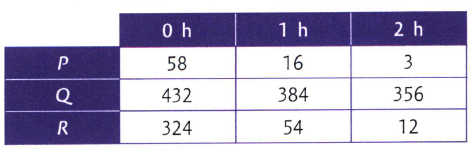
\includegraphics[width=.5\textwidth]{./img/ch2_decay_mc_2024-06-17-22-31-05.png}\par}
    從以上資料,\textbf{不可能}作出哪些結論?
    \begin{statements}
        \task $P$的致電離能力最強。
        \task $Q$不會在電場中偏轉。
        \task $R$ 的半衰期最短。
    \end{statements}
    \begin{tasks}
        \task 只有(1)和(2)
        \task 只有(1)和(3)
        \task 只有(2)和(3)
        \task (1), (2) 和 (3)
    \end{tasks}

}{A}

\newprob{1718634725}
{
    % Active Physics p88 q7
    若要使用示蹤物進行腦部造影作診斷之用,哪一 種放射源最為合適?
    \begin{tasks}
        \task [] \textbf{放出的輻射} \tab \textbf{半衰期}
        \task $\alpha$和$\beta$\tab 433年
        \task $\gamma$\tab 13.5年
        \task $\gamma$\tab 6.01小時
        \task $\beta$\tab 3.14天
    \end{tasks}

}{C}

\newprob{1718634853}
{
    % Active Physics p99 q1
    在一塊岩石中,核素$X$發生$\alpha$ 衰變而成為核素 $Y$,繼而發生$\beta$衰變而成為穩定的核素$Z$。
    \begin{align*}
        \ce{X ->[$\alpha$] Y ->[$\beta$] Z}
    \end{align*}
    在平衡狀態,即岩石中核素$Y$的數目大致不變 時,岩石的計數率為  \qty{3e4}{min^{-1}}。岩石中僅有 $X$ 和$Y$兩種放射源,$X$的半衰期為  \qty{1e5}{} 年而 $Y$的半衰期為2年。求岩石在平衡狀態時,核素 $Y$的數目。已知:1年 =  \qty{3.15e7}{s}
    \begin{tasks}
        \task \num{4.33e4}
        \task \num{2.28e10}
        \task \num{1.36e12}
        \task \num{1.15e15}
    \end{tasks}
}{B}

